\def\r{3em}
\def\angle{10}
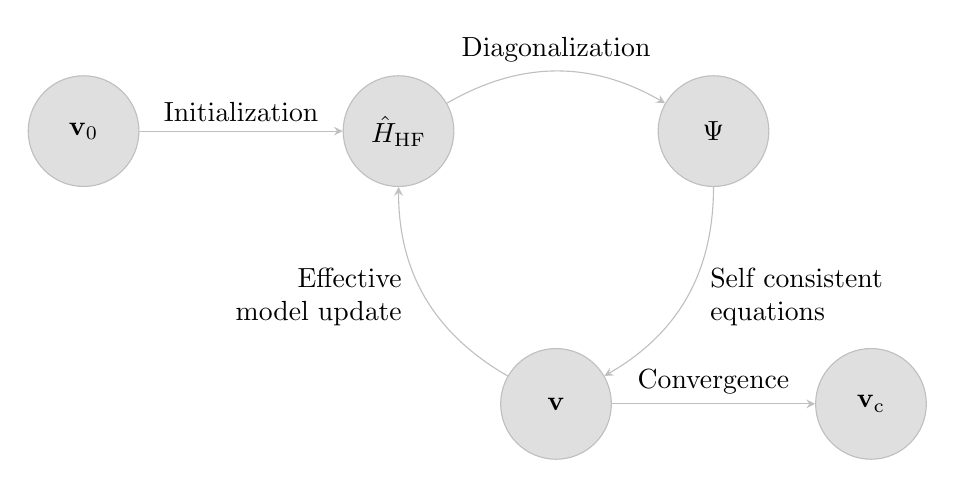
\begin{tikzpicture} 
	
	\node[
		name=i,
		circle,
		draw=lightgray,
		text=black,
		fill=lightgray!50,
		minimum size=4em
	] 
		(I) at (-4,0)
			{$\mathbf{v}_0$};
	
    \node[
        name=he,
        circle,
        draw=lightgray,
        text=black,
        fill=lightgray!50,
        minimum size=4em
    ] 
        (He) at (0,0)
            {$\hat H_\mathrm{HF}$};
            
    \node[
        name=psi,
        circle,
        draw=lightgray,
        text=black,
        fill=lightgray!50,
        minimum size=4em
    ] 
        (PSI) at (4,0)
            {$\ket{\Psi}$};
            
    \node[
        name=hfp,
        circle,
        draw=lightgray,
        text=black,
        fill=lightgray!50,
        align=center,
        minimum size=4em
    ] 
        (HFP) at (2,-3.464)
            {$\mathbf{v}$};
            
   \node[
       name=f,
       circle,
       draw=lightgray,
       text=black,
       fill=lightgray!50,
       minimum size=4em
   ] 
       (C) at (6,-3.464)
           {$\mathbf{v}_\mathrm{c}$};
         
    \draw[color=lightgray, -stealth]
    	(I) to node[above,color=black]{Initialization} (He);  
    \draw[color=lightgray, -stealth]
        (He) to[bend left]node[above,color=black]{Diagonalization} (PSI);
    \draw[color=lightgray, -stealth]
        (PSI) to[bend left]node[right,color=black,align=left,xshift=0.5em]{Self consistent\\equations} (HFP);
    \draw[color=lightgray, -stealth]
        (HFP) to[bend left]node[left,color=black,align=right,xshift=-0.5em]{Effective\\model update} (He);
    \draw[color=lightgray, -stealth]
		(HFP) to node[above,color=black]{Convergence} (C);

\end{tikzpicture}
